% (C) Brett Klamer - MIT - http://opensource.org/licenses/MIT
% Please contact me if you find any errors or make improvements
% Contact details at brettklamer.com

\documentclass[11pt,letterpaper,english,oneside]{article} % article class is a standard class
%==============================================================================
%Load Packages
%==============================================================================
\usepackage[left=1in,right=1in,top=1in,bottom=1in]{geometry} % easy page margins
\usepackage[utf8]{inputenc} % editor uses utf-8 encoding
\usepackage[T1]{fontenc} % T1 font pdf output
\usepackage{lmodern} % Latin modern roman font
\usepackage{bm, bbm} % bold and blackboard bold math symbols
\usepackage{amsmath, amsfonts, amssymb, amsthm} % math packages
\usepackage[final]{microtype} % better microtypography
\usepackage{graphicx} % for easier grahics handling
\usepackage[hidelinks, colorlinks=true, linkcolor = blue, urlcolor = blue]{hyperref} % to create hyperlinks
\usepackage{float} % tells floats to stay [H]ere!
\usepackage{enumitem} % nice lists
\usepackage{fancyhdr} % nice headers
\usepackage{caption}  % to control figure and table captions
\usepackage{booktabs} % to create nice tables

\captionsetup{width=0.9\textwidth, justification = raggedright}

%==============================================================================
% Enter name and homework title here
%==============================================================================
\author{Chris Zhanran Lin}
\title{STAT 9610: Homework 2}
\date{Due October 10, 2023 at 10:00am}

%==============================================================================
% Put title and author in PDF properties
%==============================================================================
\makeatletter % change interpretation of @
\hypersetup{pdftitle={\@title},pdfauthor={\@author}}


%==============================================================================
% Header settings
%==============================================================================
\pagestyle{fancy} % turns on fancy header styles
\fancyhf{} % clear all header and footer fields
\makeatletter
\lhead{\@author} % left header
\chead{\@title} % center header
\makeatother
\rhead{Page \thepage} % right header
\setlength{\headheight}{13.6pt} % fixes minor warning
\makeatother % change back interpretation of @

%==============================================================================
% List spacing
%==============================================================================
\setlist[itemize]{parsep=0em} % fix itemize spacing
\setlist[enumerate]{parsep=0em} % fix enumerate spacing

%==============================================================================
% Float spacing (changes spacing of tables, graphs, etc)
%==============================================================================
%\setlength{\textfloatsep}{3pt}
%\setlength{\intextsep}{3pt}

%==============================================================================
% Define Problem and Solution Environments
%==============================================================================
\theoremstyle{definition} % use definition's look
\newtheorem{problem}{Problem}
\newtheorem{solution}{Solution}
\newenvironment{prob}{\clearpage \begin{problem}\hspace{0pt}}{\end{problem}}
\newenvironment{sol}{\begin{solution}\hspace{0pt}}{\end{solution}}

\begin{document}

\maketitle

\section{Instructions}

\paragraph{Setup.} Clone this repository and open \verb|homework-2.tex| in your LaTeX editor. Use this document as a starting point for your writeup, adding your solutions between \verb|\begin{sol}| and \verb|\end{sol}|. Add R code for problem $i$ in \verb|problem-i.R| (rather than in your LaTeX report), saving your figures and tables to the \verb|figures-and-tables| folder for LaTeX import. 

\paragraph{Resources.}

Consult the \href{https://katsevich-teaching.github.io/stat-9610-fall-2023/assets/getting-started.pdf}{getting started guide} if you need to brush up on R, LaTeX, or Git, the \href{https://katsevich-teaching.github.io/stat-9610-fall-2023/assets/preparing-reports.pdf}{preparing reports guide} for guidelines on presentation quality, the \href{https://github.com/stat-9610-fall-2023/sample-homework-stat-9610}{sample homework} for an example of a completed homework repository, and \href{https://hmc-cs-131-spring2020.github.io/howtos/assignments.html}{this webpage} for more detailed instructions on using GitHub and Gradescope to complete and submit homework.

\paragraph{Programming.}

The \verb|tidyverse| paradigm for data manipulation (\verb|dplyr|) and plotting (\verb|ggplot2|) is required; points will be deducted for using base R. 

\paragraph{Grading.} Each sub-part of each problem will be worth 3 points: 0 points for no solution or completely wrong solution; 1 point for some progress; 2 points for a mostly correct solution; 3 points for a complete and correct solution modulo small flaws. The presentation quality of the solution for each problem (see the \href{https://katsevich-teaching.github.io/stat-9610-fall-2023/assets/preparing-reports.pdf}{preparing reports guide}) will be evaluated out of an additional 3 points.

\paragraph{Submission.} Compile your LaTeX report to PDF and commit your work. Then, push your work to GitHub. Finally, submit your GitHub repository to \href{https://www.gradescope.com/courses/589902}{Gradescope}.

\paragraph{Materials and collaboration.} The policy is as stated on the Syllabus:

\begin{quote}
``Students may consult all course materials, textbooks, the internet, or AI tools (e.g. ChatGPT or GitHub Copilot) to complete their homework. Students may not use solutions to problems that may be available online and/or from past iterations of the course. For each homework and exam, students must disclose all classmates with whom they collaborated, which AI tools they used, and how they used them. Failure to do so will result in a 5-point penalty. The instructor reserves the right to update this policy during the semester.''
\end{quote}

\noindent In accordance with this policy, \\

\noindent \textit{Please disclose all classmates with whom you collaborated: Zhihan Huang, Joseph Rudoler, Henry Shugart} \\

\noindent \textit{Please disclose which AI tools you used, and how you used them: ChatGPT, checking R codes} \\

\noindent \textcolor{red}{Failure to answer the above questions will result in a 5-point penalty.}

\clearpage

\begin{prob} \label{prob:likelihood}\textbf{Likelihood inference in linear regression.} \\

    \noindent Let's consider the usual linear regression setup. Given a full-rank $n \times p$ model matrix $\bm X$, a coefficient vector $\bm \beta \in \mathbb R^p$, and a noise variance $\sigma^2 > 0$, suppose
    \begin{equation}
    \bm y = \bm X \bm \beta + \bm \epsilon, \quad \bm \epsilon \sim N(0, \sigma^2 \bm I_n).
    \label{eq:linear-model}
    \end{equation}
    The goal of this problem is to connect linear regression inference with classical likelihood-based inference (below is a quick refresher).
    
    \begin{enumerate}
    \item[(a)] For the sake of simplicity, let's start by assuming $\sigma^2$ is known. Under the fixed-design model, why does the linear regression model~\eqref{eq:linear-model} not fit into the classical inferential setup~\eqref{eq:iid-sampling}? Write the linear model in as close a form as possible to~\eqref{eq:iid-sampling}.
    
    \item[(b)] Continue assuming that $\sigma^2$ is known. Why does the Fisher information~\eqref{eq:fisher-info} not immediately make sense for the linear regression model? Propose and compute an analog to this quantity, and using this quantity exhibit a result analogous to the asymptotic normality~\eqref{eq:asymptotic-normality}.
    
    \item[(c)] Now assume that neither $\bm{\beta}$ nor $\sigma^2$ is known. Derive the maximum likelihood estimates for $(\bm \beta, \sigma^2)$. How do these compare to the estimates $(\bm{\widehat \beta}, \widehat \sigma^2)$ discussed in class?
    
    \item[(d)] Continuing to assume that neither $\bm{\beta}$ nor $\sigma^2$ is known, consider the null hypothesis $H_0: \bm{\beta}_S = \bm 0$ for some $S \subseteq \{1, \dots, p\}$. Write this hypothesis in the form~\eqref{eq:general-null-hypothesis}, and derive the likelihood ratio test for this hypothesis. Discuss the connection of this test with the $F$-test.
    
    \end{enumerate}
    
    \noindent\fbox{\begin{minipage}{\textwidth}
    \paragraph{Refresher on likelihood inference.} In classical likelihood inference, we have observations 
    \begin{equation}
    y_i \overset{\text{i.i.d.}}\sim p_{\bm \theta}, \quad i = 1, \dots, n
    \label{eq:iid-sampling}
    \end{equation}
    from some model parameterized by a vector $\bm \theta \in \Theta \subseteq \mathbb R^d$. Under regularity conditions, the maximum likelihood estimate $\bm{\widehat \theta}_n$ is known to converge to a normal distribution centered at its true value:
    \begin{equation}
    \sqrt n(\bm{\widehat \theta}_n - \bm \theta) \overset d \rightarrow N(0, \bm I(\bm \theta)^{-1}),
    \label{eq:asymptotic-normality}
    \end{equation}
    where 
    \begin{equation}
    \bm I(\bm \theta) \equiv -\mathbb E_{\bm \theta}\left[\frac{\partial^2}{\partial \bm \theta^2} \log p_{\bm \theta}(y) \right]
    \label{eq:fisher-info}
    \end{equation}
    is the per-observation Fisher information matrix.
    Furthermore, an optimal test of the null hypothesis 
    \begin{equation}
    H_0: \bm \theta \in \Theta_0 \quad \text{versus} \quad H_1: \bm \theta \in \Theta_1 \setminus \Theta_0
    \label{eq:general-null-hypothesis}
    \end{equation}
    for some $\Theta_0 \subseteq \Theta_1 \subseteq \Theta$ is the likelihood ratio test based on the test statistic
    \begin{equation}
    \Lambda = \frac{\max_{\bm \theta \in \Theta_1}\prod_{i = 1}^n p_{\bm \theta}(y_i)}{\max_{\bm \theta \in \Theta_0}\prod_{i = 1}^n p_{\bm \theta}(y_i)}.
    \end{equation}
    Under $H_0$, we have the convergence 
    \begin{equation}
    2 \log \Lambda \overset d \rightarrow \chi^2_k, \quad \text{where} \quad k \equiv \text{dim}(\Theta_1) - \text{dim}(\Theta_0).
    \end{equation}
    \end{minipage}
    }
    \end{prob}
    
    \begin{sol}
    \begin{itemize}
        \item[(a)] Because we have covariates $\bm X$ here. Our observations are actually can be viewed as
        $$
            y_i = \bm X_i^T \bm \beta + \epsilon_i \sim \mathcal{N}(\bm X_i^T \bm \beta, \sigma^2 \bm I_n)
        $$
        independently for $i \in [n]$. This is a model parameterized by a vector $\bm \beta$, while, at the same time, depends on the covariate $\bm X_i$.
        \item[(b)] Because we need to consider covariates in each observations $y_i$ under the regression model. We can
        write down the density function
        $$
            p_\beta(X_i, y_i) = \frac{1}{\sqrt{2 \pi}\sigma}\text{exp}\{-\frac{1}{2\sigma^2}(y_i - \bm X_i^T \beta)^2\},
        $$
        then 
        \begin{align*}
            \bm I(\bm \beta) &= -\mathbb E_{\bm \beta}\left[\frac{\partial^2}{\partial \bm \beta^2} \log p_{\bm \beta}(\bm X, \bm y) \right] \\
            &= -\mathbb E_{ \bm \beta}\left[\frac{\partial^2}{\partial \bm \beta^2} \log \prod_{i=1}^n p_{\bm \beta}(\bm X_i,  y_i) \right] \\
            &= -\mathbb E_{ \bm \beta}\frac{\partial^2}{\partial \bm \beta^2}\left( -\frac{1}{2 \sigma^2} \sum_{i=1}^n (y_i - \bm X_i^T \bm \beta) \right) \\
            &= \frac{1}{\sigma^2} E_{ \bm \beta} \sum_{i=1}^n \bm X_i \bm X_i^T = \frac{1}{\sigma^2}(\bm X^T \bm X).
        \end{align*}
        Then we have 
        $$
            \sqrt{n}(\hat{\bm \beta}_n - \bm \beta) \sim \mathcal{N}(0, n\bm I (\bm \beta)^{-1}) = \mathcal{N}(0, n\sigma^2(\bm X^T \bm X)^{-1})
        $$
        For asymptotic property, if we have
        $$
           \lim_{n \rightarrow \infty}\sigma^2(\frac{1}{n}\bm X^T \bm X)^{-1} =  \sigma^2 (\mathbb E [\bm x \bm x^T ])^{-1}
        $$
        then we may derive $\sqrt{n}(\hat{\bm \beta}_n - \bm \beta) \rightarrow \mathcal{N}(0, \sigma^2 (\mathbb E [\bm x \bm x^T])^{-1})$.

    \item[(c)] Let
    $$
        L(\bm \beta, \sigma^2) = \left(\frac{1}{\sqrt{2 \pi}\sigma}\right)^n exp\left\{-\frac{1}{2\sigma^2}\sum_{i=1}^n(y_i - \bm X_i^T \bm \beta)^2\right\},
    $$
    and
    $$
        l(\bm \beta, \sigma^2) = \text{ln}L(\bm \beta, \sigma^2) = - \text{ln} \sqrt{2 \pi} \sigma - \frac{1}{2\sigma^2} \sum_{i=1}^n (y_i - \bm X_i^T \bm \beta)^2.
    $$
    Take the maximum likelihood estimate by derivation, let
    $$
        \frac{\partial l}{\partial \bm \beta} = \frac{1}{\sigma^2} \sum_{i=1}^n (y_i - \bm X_i^T \bm \beta) \bm X_i = 0
    $$
    we obtain $\hat{\bm \beta} = (\bm X^T \bm X)^{-1} \bm X y$. Similarly, take  $
        \frac{\partial l}{\partial \sigma} = 0
    $
    we can derive $\widehat{\sigma^2} = \frac{1}{n}\sum_{i=1}^n(y_i - \bm X_i^T \bm \beta)^2$.

    Comparing to the estimates discussed in class, we can find that the $\hat{\bm \beta}$ keeps the same, while the coefficient of $\widehat{\sigma^2}$ changes from $\frac{1}{n-p}$ to $\frac{1}{n}$ (though they share the same asymptotic results).

    \item[(d)] Consider $H_0: \bm \beta \in \Theta_0 =  \{ \beta: \beta_S = \bm 0\}$ and $H_1 : \bm \beta \in \Theta_1 \setminus \Theta_0 = \{ \beta: \beta_S \neq \bm 0\} $, obviously for $\Theta_1$, the maximum is achieved at the MLE estimator, which is 
    $$
        l(\hat{\bm \beta}, \widehat{\sigma^2}) = -\frac{n}{2}\log(\frac{2 \pi}{n}) - \frac{n}{2}\log(RSS_1) - \frac{n}{2},
    $$
    for $RSS_1 = \|y - \bm X\hat{\bm \beta}\|^2$. Similarly, under $\Theta_0$ we can view the problem as regression using the covariates with indexes $-S$, and the maximum is derived by
    $$
        l(\hat{\bm \beta_{-S}}, \widehat{\sigma_{-S}^2}) = -\frac{n}{2}\log(\frac{2 \pi}{n}) - \frac{n}{2}\log(RSS_0) - \frac{n}{2}
    $$
    with $RSS_0 = \|y - \bm X_{\dot,-S}\hat{\bm \beta_{-S}}\|^2$.
    Thus we have
    $$
    \Lambda = \frac{\max_{\bm \theta \in \Theta_1}\prod_{i = 1}^n p_{\bm \theta}(y_i)}{\max_{\bm \theta \in \Theta_0}\prod_{i = 1}^n p_{\bm \theta}(y_i)} = \frac{\text{exp}\{-\frac{n}{2}\log(RSS_1)\}}{\text{exp}\{-\frac{n}{2}\log(RSS_0)\}} = \left(\frac{RSS_0}{RSS_1}\right)^{n/2},
    $$
    then $$2\log \Lambda = n \log \left(\frac{RSS_0}{RSS_1}\right) \rightarrow \chi_k^2$$ with $k \equiv \text{dim}(\Theta_1) - \text{dim}(\Theta_0) = |S|$. The form is close to the F-test, while $\left(\frac{RSS_0}{RSS_1}\right)$ is used by a log transformation (Although $\chi^2$ distribution is not a F-distribution).
    \end{itemize}
    
    \end{sol}
    
    \begin{prob} \textbf{Relationships among $t$-tests, $F$-tests, and $R^2$.} \\
    
    \noindent Consider the linear regression model~\eqref{eq:linear-model}, such that $\bm x_{*,0} = \bm 1_n$ is an intercept term.
    
    \begin{itemize}
    \item[(a)] Relate the $R^2$ of the linear regression to the $F$-statistic for a certain hypothesis test. What is the corresponding null hypothesis? What is the null distribution of the $F$-statistic? Are $R^2$ and $F$ positively or negative related, and why does this make sense?
    
    \item[(b)] Use the relationship found in part (a) to simulate the null distribution of the $R^2$ by repeatedly sampling from an $F$ distribution (via \verb|rf|). Fix $n = 100$ and try $p \in \{2, 25, 50, 75, 99\}$. Comment on these null distributions, how they change as a function of $p$, and why. 
    
    \item[(c)] Consider the null hypothesis $H_0: \beta_j = 0$, which can be tested using either a $t$-test or an $F$-test. Write down the corresponding $t$ and $F$ statistics, and prove that the latter is the square of the former. 
    
    \item[(d)] Now suppose we are interested in testing the null hypothesis $H_0: \bm \beta_{\text{-}0} = \bm 0$ (here, $\bm \beta_{\text{-}0} \equiv (\beta_1, \dots, \beta_{p-1})^T$). One way of going about this is to start with the usual test statistic $t(\bm c)$ for the null hypothesis $H_0: \bm c^T \bm \beta_{\text{-}0} = 0$, and then maximize over all $\bm c \in \mathbb R^{p-1}$:
    \begin{equation}
    t_{\max} \equiv \max_{\bm c \in \mathbb R^{p-1}} t(\bm c).
    \end{equation}
    What is the null distribution of $t_{\max}^2$? What $F$-statistic is $t_{\max}^2$ equivalent to? How does the null distribution of $t_{\max}^2$ compare to that of $t(\bm c)^2$?
    
    \end{itemize}
    
    \end{prob}
    \begin{sol}
    \begin{itemize}
        \item[(a)]
        We have 
        $$
R^2 = 1 - \frac{\|y - \bm X \bm \beta\|^2}{\|y - \Bar{y}\textbf{1}_n\|^2},
        $$
        then considering F-test for $H_0: \bm \beta_S = 0$ for $S = \{1,2,\ldots,p\}$ as in problem 1(c), we will have
        $$
            F = \frac{\frac{\|y - \Bar{y}\textbf{1}_n\|^2 - \|y - \bm X \hat{\bm \beta}\|^2}{p-1}}{\frac{\|y - \bm X \hat{\bm \beta}\|^2}{n-p}} = \frac{n-p}{p-1} \cdot \frac{R^2}{1 - R^2}.
        $$
        $F$ and $R^2$ are positively related. Intuitively, as $R^2$ refers to the proportion of variance that has been explained by the model, $F$ shows the significance that the covariates explain the respond. They should be somehow positively related.

        \item[(b)] Consider that $$
            R^2 = \frac{F}{F + \frac{n-p}{p-1}}
        $$
        from (a), we can sample $F$ distribution and get null-distribution simulation of $R^2$. The simulations are shown below.
        \begin{figure}
    % \centering
\begin{minipage}[ht]{0.5\linewidth}
\centering
    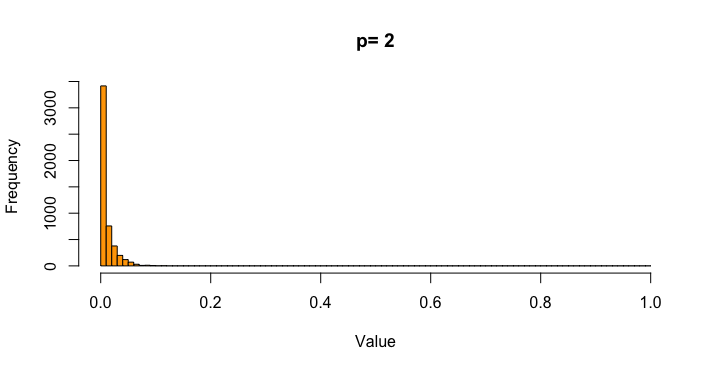
\includegraphics[height = 5cm, width =8.5cm]{figures-and-tables/2-2-1.png}
    \end{minipage}
\begin{minipage}[ht]{0.5\linewidth}
   \centering
    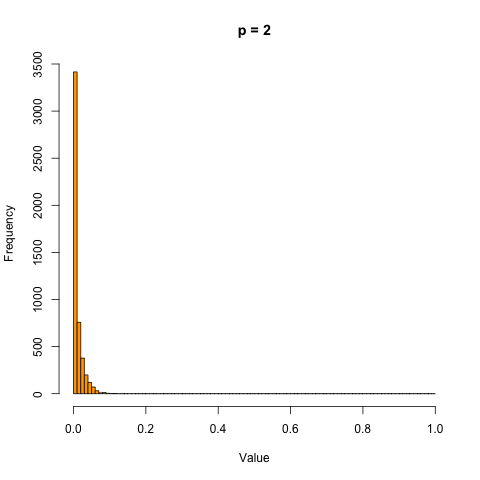
\includegraphics[height = 5cm, width =8.5cm]{figures-and-tables/2-2-2.png}
    \end{minipage}
    % \qquad
% \caption{}
% \label{fig:coordinate}
\end{figure}

\begin{figure}
\begin{minipage}[ht]{0.5\linewidth}
\centering
    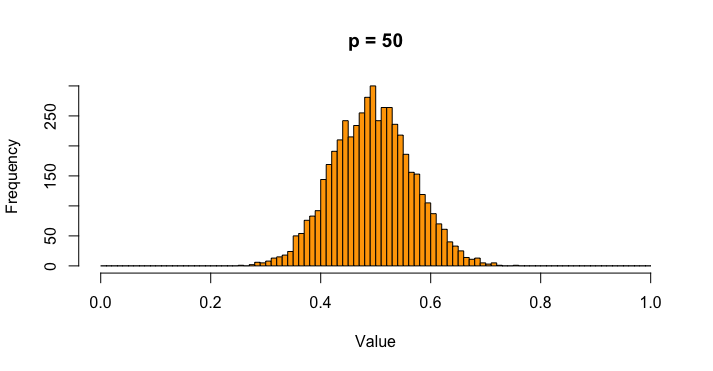
\includegraphics[height = 5cm, width =8.5cm]{figures-and-tables/2-2-3.png}
    \end{minipage}
\begin{minipage}[ht]{0.5\linewidth}
   \centering
    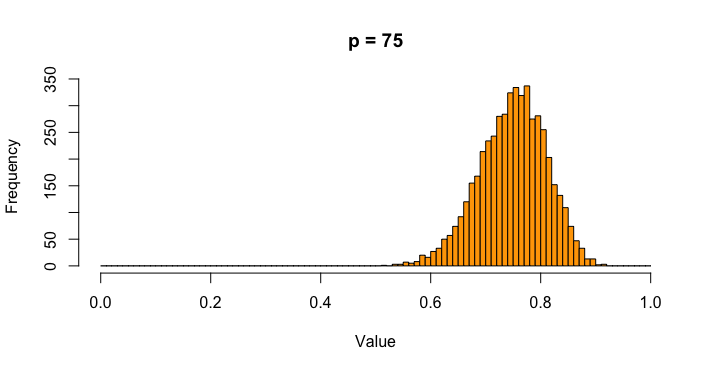
\includegraphics[height = 5cm, width =8.5cm]{figures-and-tables/2-2-4.png}
    \end{minipage}
    % \qquad
% \caption{}
% \label{fig:coordinate}
\end{figure}


\begin{figure}
\begin{minipage}[ht]{0.5\linewidth}
\centering
    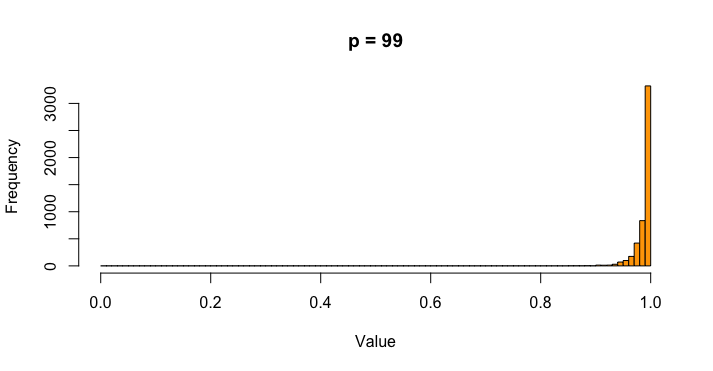
\includegraphics[height = 5cm, width =8.5cm]{figures-and-tables/2-2-5.png}
    \end{minipage}
    % \qquad
% \caption{}
% \label{fig:coordinate}
\end{figure}

For each $p$ we generate $50000$ samples to get the frequency result.
We can see that the distribution is on $[0,1]$. As $p$ increases, the distribution goes  to the right side (more close to $1$). Intuitively, larger $p$ refers to more covariates involved in the model, thus we can obtain better explanations of the total variance.

\item[(c)] We can write down the t-statistic as
$$
        t = \frac{\hat{\beta}_j}{\hat{\sigma}\sqrt{v_j}} = 
        \frac{\hat{\beta}_j}{\hat{\sigma}\sqrt{(\bm X^T \bm X)_{jj}^{-1}}},
$$
while the F-statistic is
$$
    F = \frac{\|\bm X_{\dot,-j}\hat{\bm \beta}_{-j} - \bm X \hat{\bm \beta}\|^2}{\hat{\sigma}^2} = \frac{\hat{\beta}_j^2}{\hat{\sigma}^2{(\bm X^T \bm X)_{jj}^{-1}}}.
$$
Thus the latter is obviously the square of the former.

\item[(d)] Consider $\bm c^T \bm \beta_{-0} = 0$, then we have
$$
    t(\bm c) = \frac{\bm c^T \hat{\bm \beta}_{-0}}{\hat{\sigma}\sqrt{\bm c^T (\bm X^T \bm X)_{-1, -1}^{-1} \bm c}}.
$$
Following this, we may derive the maximimal 
$$
 t_{max}^2 = \max t(\bm c)^2 = \max \left( \frac{\bm c^T \hat{\bm \beta}_{-0}}{\hat{\sigma}\sqrt{\bm c^T (\bm X^T \bm X)_{-1, -1}^{-1} \bm c}} \right) = \frac{1}{\hat{\sigma}^2}{\hat{\bm \beta}_{-0}^T (\bm X^T \bm X)_{-1, -1} \hat{\bm \beta}_{-0}}
$$
with $\bm c = \hat{\bm \beta}_{-0}$. The distribution turns out to be $\frac{p-1}{n-p}F_{p-1, n-p}$, which shares the same form with the F-statistic in (a) by multiplying a constant. Obviously we have $t_{max}^2 \ge t(\bm c)^2$ and $t_{max}^2$ would be more related to F-statistics as shown.
    \end{itemize}
    \end{sol}






    
    \begin{prob} \label{prob:data}\textbf{Case study: Violent crime.}
    
    \noindent The \texttt{Statewide\_crime.tsv} file contains information on the number of violent crimes and murders for each U.S. state in 2015, as well as three socioeconomic indicators: percent living in metropolitan areas, high school graduation rate, and poverty rate (Table~\ref{tab:crime-data}).

    \begin{table}[!h]

\caption{\label{tab:crime-data}The first five rows of the crime data.}
\centering
\begin{tabular}[t]{lrrrrr}
\toprule
STATE & Violent & Murder & Metro & HighSchool & Poverty\\
\midrule
AK & 593 & 6 & 65.6 & 90.2 & 8.0\\
AL & 430 & 7 & 55.4 & 82.4 & 13.7\\
AR & 456 & 6 & 52.5 & 79.2 & 12.1\\
AZ & 513 & 8 & 88.2 & 84.4 & 11.9\\
CA & 579 & 7 & 94.4 & 81.3 & 10.5\\
\bottomrule
\end{tabular}
\end{table}


    \noindent The goal of this problem is to study the relationship between the three socioeconomic indicators and the per capita violent crime rate.
    
    \begin{itemize}
    \item[(a)] These data contain the total number of violent crimes per state, but it is more meaningful to model violent crime rate per capita. To this end, go online to find a table of current populations for each state. Augment \verb|crime_data| with a new variable called \verb|Pop| with this population information (see \verb|left_join()| from the \verb|dplyr| package) and create a new variable called \verb|CrimeRate| defined as \verb|CrimeRate = Violent/Pop| (see \verb|mutate()| from the \verb|dplyr| package).
    
    \item[(b)] Explore the variation and covariation among the variables \verb|CrimeRate|, \verb|Metro|, \verb|HighSchool|, \verb|Poverty| with the help of visualizations and summary statistics.
    
    \item[(c)] Construct linear model based hypothesis tests and confidence intervals associated with the relationship between \verb|CrimeRate| and the three socioeconomic variables, including any relevant tables or plots in your LaTeX report. Discuss the results in technical terms.
    
    \item[(d)] Discuss your interpretation of the results from part (c) in language that a policymaker could comprehend, including any caveats or limitations of the analysis. Comment on what other data you might want to gather for a more sophisticated analysis of violent crime.
    
    \end{itemize}
    
    \end{prob}
    \begin{sol}
    \begin{itemize}
        \item[(a)] See the codes.

        \item[(b)] 
        The summary is shown in Table \ref{table:summary} and the variance is in Table \ref{table:var}. The covariance matrix is shown in Figure \ref{fig:correlation}. It looks like the Poverty is more (positively) related to CrimeRate, while it (negatively) relates to the HighSchool number, which is totally reasonable. A scatterplot is shown in Figure \ref{fig:scatterplot}. It looks like there is no significant linear relationship between CrimeRate and the other three variables (separately).
        \begin{table}[h]
\centering
\begin{tabular}{llll}
  \hline
  CrimeRate &     Metro &   HighSchool &    Poverty \\ 
  \hline
Min.   :1.289e-07   & Min.   : 38.20   & Min.   :78.30   & Min.   : 5.100   \\ 
  1st Qu.:2.373e-06   & 1st Qu.: 60.80   & 1st Qu.:84.00   & 1st Qu.: 7.300   \\ 
  Median :5.525e-06   & Median : 71.60   & Median :87.20   & Median : 8.500   \\ 
  Mean   :1.151e-05   & Mean   : 72.25   & Mean   :86.46   & Mean   : 9.506   \\ 
  3rd Qu.:1.080e-05   & 3rd Qu.: 86.80   & 3rd Qu.:88.80   & 3rd Qu.:10.750   \\ 
  Max.   :8.559e-05   & Max.   :100.00   & Max.   :92.30   & Max.   :18.500   \\ 
   \hline
\end{tabular}
\caption{Summary Table} 
\label{table:summary}
\end{table}
\begin{table}[h]
\centering
\begin{tabular}{rr}
  \hline
 & Variance \\ 
  \hline
CrimeRate     &    3.038195e-10 \\
Metro         &    2.333529e+02 \\
HighSchool    &    1.307638e+01 \\
Poverty       &    9.794165e+00 \\
   \hline
\end{tabular}
\caption{Variance} 
\label{table:var}
\end{table}
    
   
\begin{figure}
      \centering
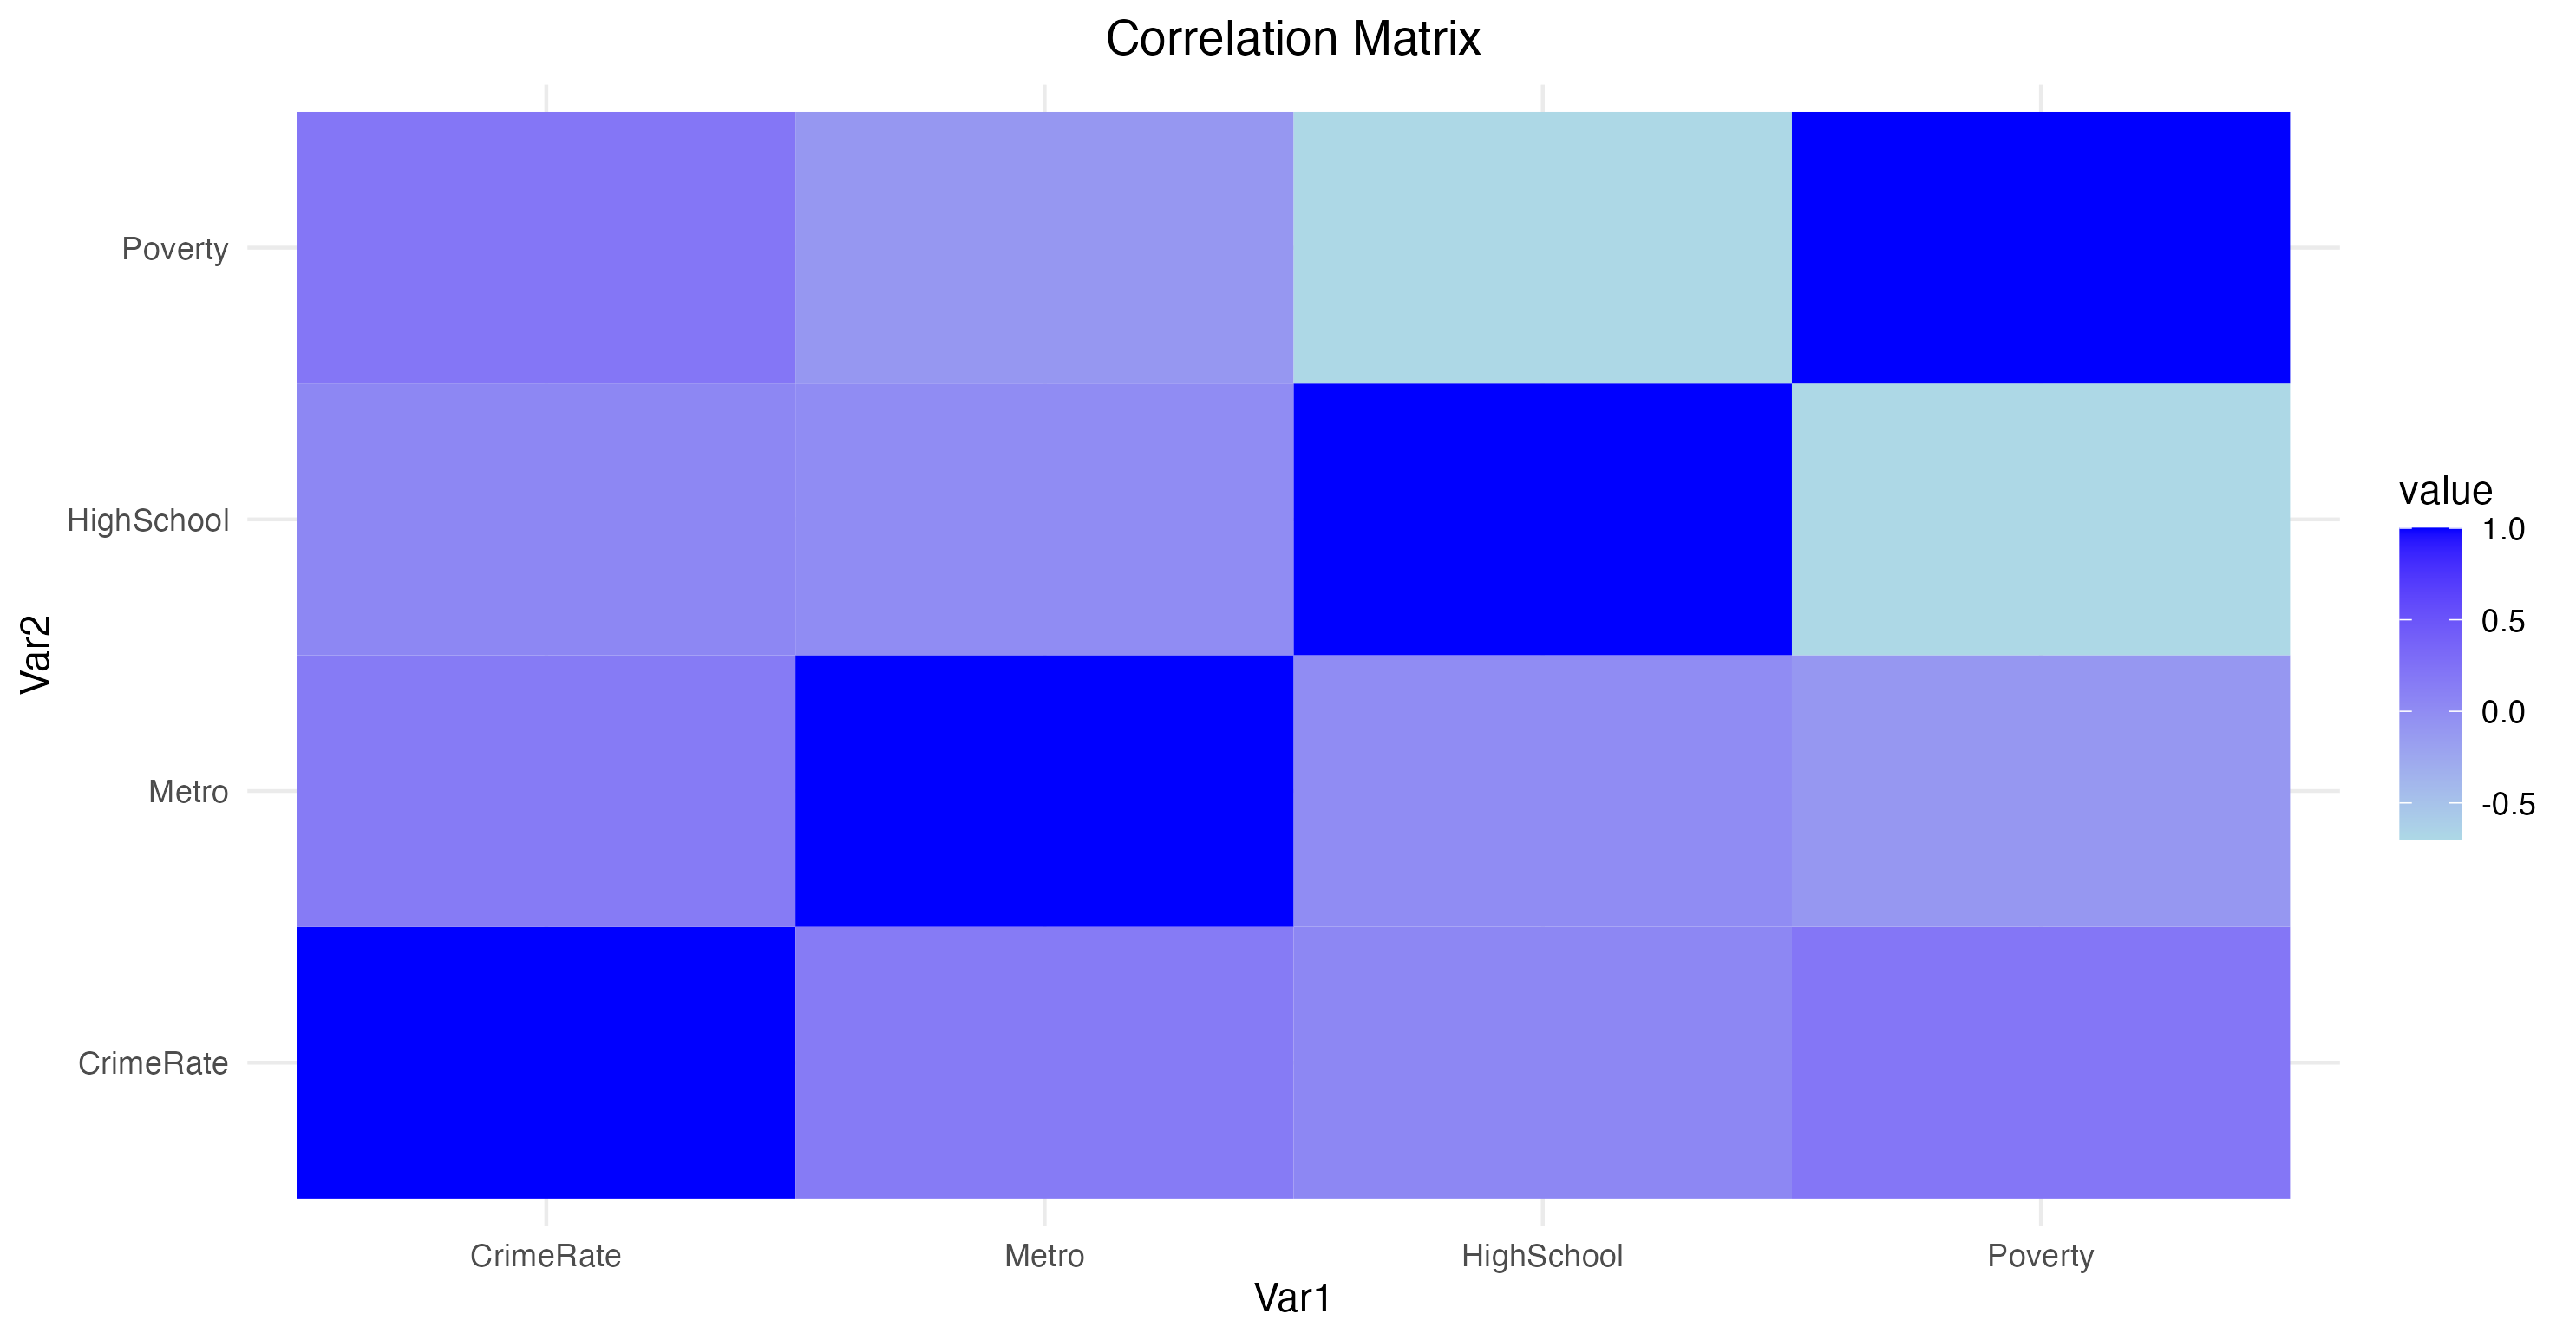
\includegraphics[width=0.53\textwidth, height=0.4\textwidth]{figures-and-tables/3-2-correlation.png} % Adjust the width as needed
  \caption{Correlation Matrix}
  \label{fig:correlation}
\end{figure}

\begin{figure}
      \centering
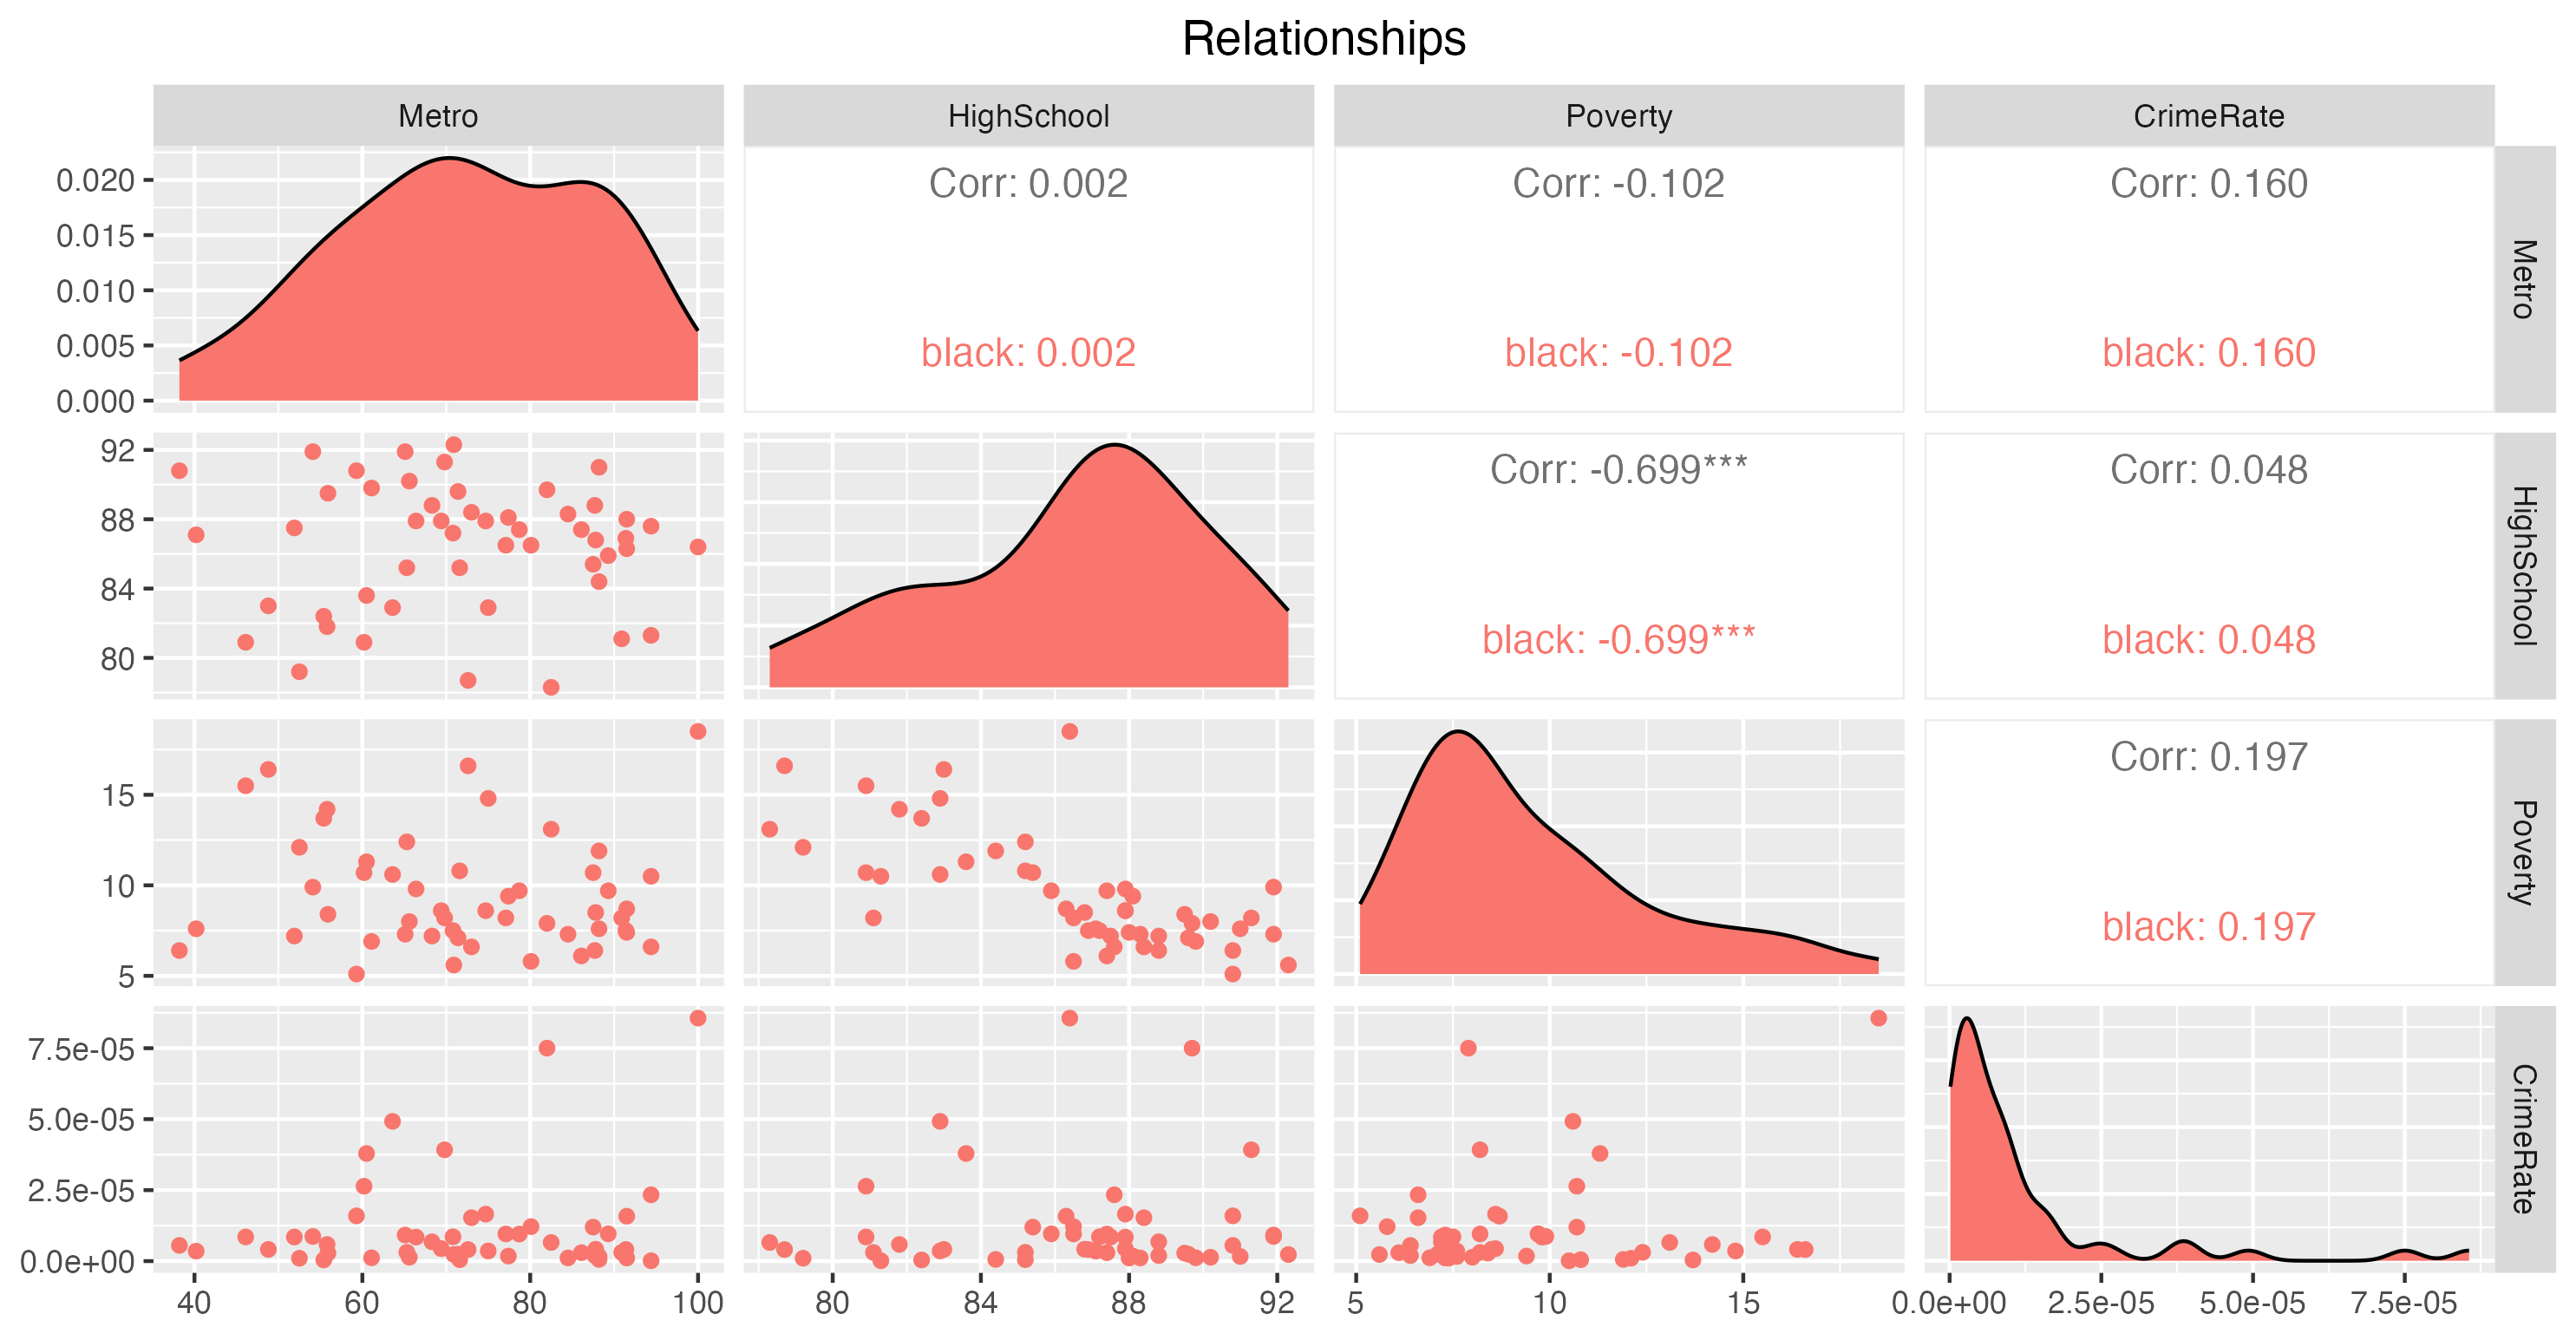
\includegraphics[width=0.84\textwidth, height=0.45\textwidth]{figures-and-tables/3-2-scatterplot.png} % Adjust the width as needed
  \caption{Scatterplot}
  \label{fig:scatterplot}
\end{figure}

\item[(c)] We construct linear tests separately on the linear relationship of CrimeRate and the other three socioeconomic variables. 


\begin{table}[h]
\centering
\begin{tabular}{rllll}
  \hline
 & Estimate & Std. Error & t value & Pr($>$$|$t$|$) \\ 
  \hline
(Intercept) & -1.714230e-06 & 1.187644e-05 & -0.1443387 & 0.8858251 \\ 
  Metro &  1.830758e-07 & 1.608940e-07 &  1.1378655 & 0.2607099 \\ 
   \hline
\end{tabular}
\caption{}
\label{tab:1}
\end{table}



\begin{table}[h]
\centering
\begin{tabular}{rllll}
  \hline
 & Estimate & Std. Error & t value & Pr($>$$|$t$|$) \\ 
  \hline
(Intercept) & -8.590027e-06 & 5.951977e-05 & -0.1443222 & 0.885838 \\ 
  HighSchool &  2.325029e-07 & 6.877968e-07 &  0.3380401 & 0.736777 \\ 
   \hline
\end{tabular}
\caption{}
\label{tab:2}
\end{table}


\begin{table}[h]
\centering
\begin{tabular}{rllll}
  \hline
 & Estimate & Std. Error & t value & Pr($>$$|$t$|$) \\ 
  \hline
(Intercept) & 1.081375e-06 & 7.799201e-06 & 0.138652 & 0.8902934 \\ 
  Poverty & 1.097367e-06 & 7.800608e-07 & 1.406771 & 0.1658065 \\ 
   \hline
\end{tabular}
\caption{}
\label{tab:3}
\end{table}

In Table \ref{tab:1}, \ref{tab:2}, \ref{tab:3} shows that for each separate variable, we don't have significant evidence to reject the null hypothesis $H_0: \beta_j = 0$ (since the p-values $0.261, 0.737, 0.166$ all far beyond $0.05$). However, we can do linear model based hypothesis test on the three variables simultanously as shown in Table \ref{tab:4}. The p-value for the whole model is $0.05276$ (not shown in the table, see in the codes), which is slightly over than $0.05$ (as a common boundary), showing that the whole linear relationship is in an indistinct boundary; the p-values for the Poverty and HighSchool terms are smaller than $0.05$, which shows significant evidence for us to reject the hypothesis $\beta_{\text{poverty}} = 0$ and $\beta_{\text{highschool}}$. The confidence intervals could also be seen in the table through standard errors. And a intuitive visuallization could be refered to Figure \ref{fig:scatterplot}. When we construct a linear model based on both the three variables, the HighSchool and Poverty items show significant linear relationship with the outcome CrimeRate.

\begin{table}[h]
\centering
\begin{tabular}{rllll}
  \hline
 & Estimate & Std. Error & t value & Pr($>$$|$t$|$) \\ 
  \hline
(Intercept) & -1.951633e-04 & 8.803279e-05 & -2.216938 & 0.03150170 \\ 
  Poverty &  2.742104e-06 & 1.057978e-06 &  2.591834 & 0.01268023 \\ 
  HighSchool &  1.888735e-06 & 9.108256e-07 &  2.073651 & 0.04361672 \\ 
  Metro &  2.395158e-07 & 1.550299e-07 &  1.544965 & 0.12906211 \\ 
   \hline
\end{tabular}
\caption{}
\label{tab:4}
\end{table}

\item[(d)] By our statistical model, it is shown that the HighSchool and Poverty items might have (linear) relationship with the CrimeRate, while the Metro number seems less relative. We need to improve economical conditions (of cities) and educational guidance to enhance the population's quality, which might further alleviate the crime rate. The limitations (or, caveats) might be: (1) too few variables to conduct conclusions, and the significance depends on the model we take. (2) The terms we considered might be biased from practical settings, e.g., population and crime rate per captia might not be the only way to depict average effect violent crimes.

Some other data we may want to gather might be: range of metropolitan areas (square miles), repeat-crime data, high-school-related violent rate, which might help us have a fine-grain analysis on the crime issues. At the same time, we may want goverment policy data (e.g., gun-related policy), GDP, etc, which could provide us with more variables to do better analysis.

\end{itemize}
 \end{sol}

\end{document}